\section{A* Search}\label{sec:astar}

%\begin{figure}[!t]
%\centering
%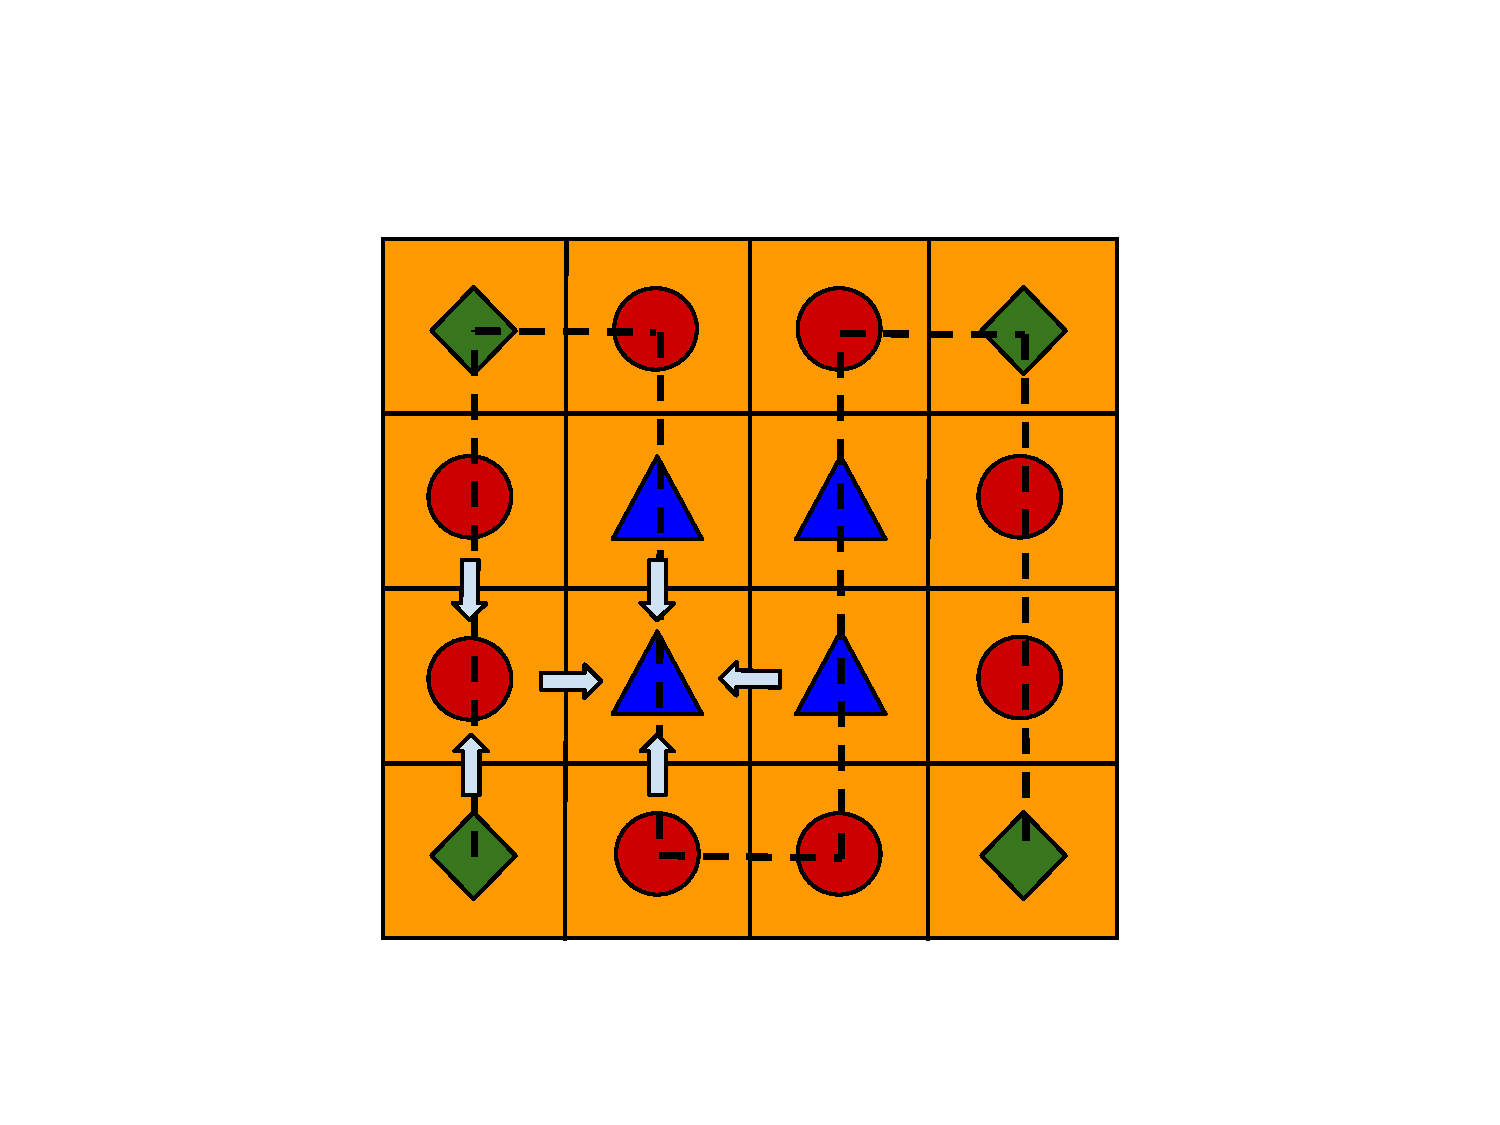
\includegraphics[scale=.35]{img/celltype.pdf}
%\caption{We use different shapes to represent different cell types. We can see that it is not possible to step into a triangle cell in the memoryless deterministic reflex agent case, because an agent cannot take 2 different actions in circle cells, but which is necessary to get into the center.}
%\label{fig:celltypes}
%\end{figure}

We implement the A* search algorithm for finding the paths between initial states to a given goal state in the problem of Tower of Corvallis. It is summarized in figure \ref{alg1}.

\begin{algorithm}[H]
\caption{A* Search}
\label{alg1}
\begin{algorithmic}
\STATE exploredSet = $\emptyset$ 
\STATE frontier = [initialPath]
\WHILE{number(explored) $<$ NMAX}
\IF{frontier == $\emptyset$}
    \RETURN FALSE
\ENDIF
\STATE path = frontier.pop()
\STATE state = path[0]
\IF{state == goalState}
    \RETURN path
\ENDIF
\FOR{action in state.validActions()}
    \FOR{newState in action.results()}
        \STATE newPath = path + newState
        \IF{ismember(frontier,newPath) == FALSE}
            \STATE frontier.push(newPath)
        \ENDIF
    \ENDFOR
\ENDFOR
\ENDWHILE
\end{algorithmic}
\end{algorithm}

For implementing the frontier, we use the priority queue, which is actually a heap data structure. We use a callback function $f(state) = g(state) + h(state)$ as the priority, where $g(state)$ is the length of the path and $h(state)$ is the heuristic for estimating the distance between the current state to the goal state. We will analyze several admissble and non-admissble heuristics in section \ref{sec:exp}.

